\section{Profile Select Activity}
This section will explain the Profile Select Activity and how it makes some of the external architecture for others to use.

The final implementation of the design is made so it is simple and easy to use. What can be seen on this screen is the giraf logo and colors to secure consistency and then the children connected to the currently logged in guardian profile.

This can be seen in \autoref{fig:profile-select-activity_2} and in \autoref{fig:profile-select-activity_1} on page \pageref{fig:profile-select-activity_1}.

\begin{figure}[h!]
	\centering
	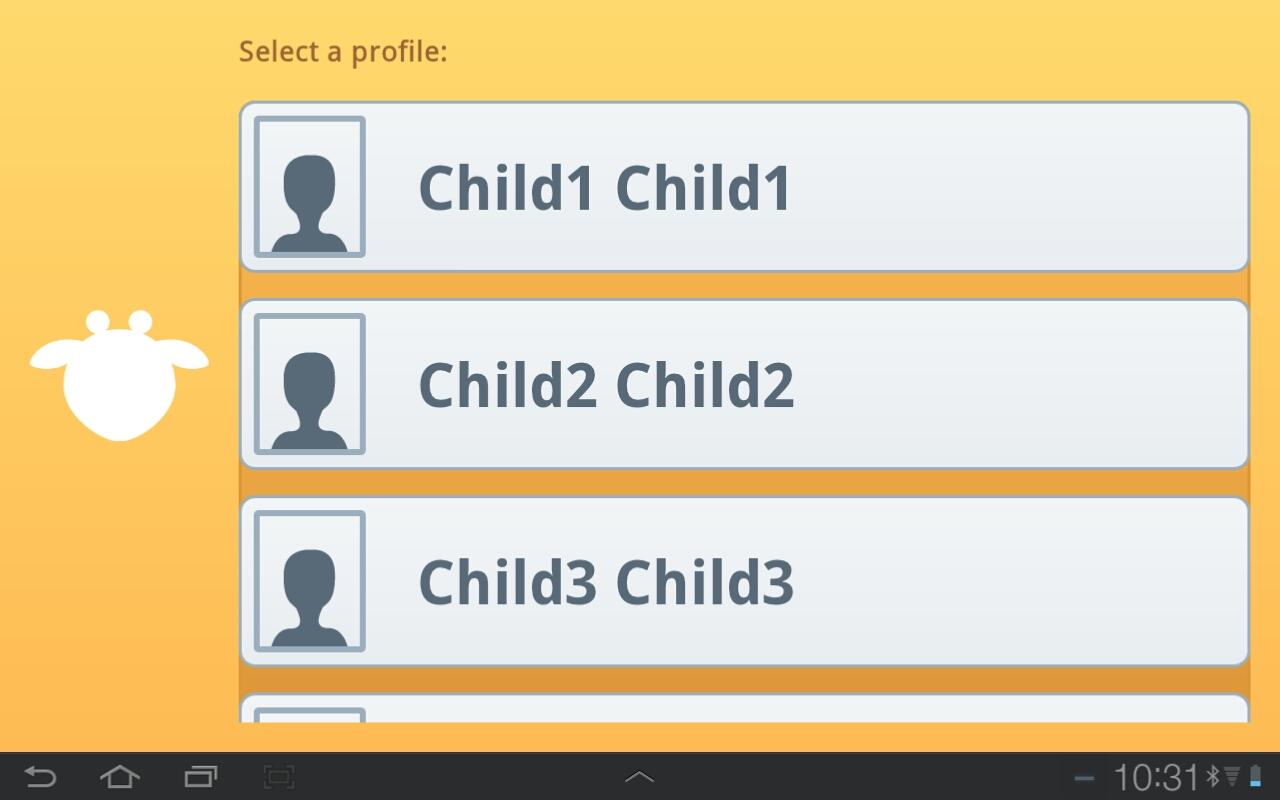
\includegraphics[scale=0.3]{gfx/profile-select-activity_2.jpg}
	\caption{Landscape profile select activity screenshot}
	\label{fig:profile-select-activity_2}
\end{figure}

The external architecture is build using intents which Android have defined as ``An intent is an abstract description of an operation to be performed.'' \citep{android:intent}. These intents can hold almost any data Java can handle and is easy to use. The \verb + putExtra() + method puts a data type e.g. long in the intent with some kind of tag, which is of the type \verb + String +. This activity puts three extra attributes in the intent before calling \verb + startActivity + for the intent with the selected application in it. These are a \verb +childID+ which holds the id of the selected child, \verb +mGuardianID+ which holdes the current logged in guardians id and the color which the user have choosen for the application icon. All other applications in giraf can look at the intent they were started with and use this information. How the intent is build can be seen in \autoref{lst:profileActivity}.

\begin{lstlisting}[style=sourceCode, language=JAVA, caption=How the launcher makes the intent for launching an application, label=lst:profileActivity] 
listOfChildren.setOnItemClickListener(new OnItemClickListener() {
			public void onItemClick(AdapterView<?> parent, View view, int position, long id) {
				final long childID = ((Profile) parent.getAdapter().getItem(position)).getId();

				Intent intent = new Intent(Intent.ACTION_MAIN);
				intent.addCategory(Intent.CATEGORY_LAUNCHER);
				intent.setComponent(new ComponentName(mPackageName, mActivityName));
				intent.setFlags(Intent.FLAG_ACTIVITY_NEW_TASK
						| Intent.FLAG_ACTIVITY_RESET_TASK_IF_NEEDED);

				intent.putExtra(Data.CHILDID, childID);
				intent.putExtra(Data.GUARDIANID, mGuardianID);
				intent.putExtra(Data.APP_COLOR, mAppColor);

				startActivity(intent);
			}
		});
\end{lstlisting}